% cd /storage/emulated/0/Documents/documents/latex/1920/Grade-10/1st/tangent-lines-and-tangent-circles && pdflatex ps-tangent-lines-and-tangent-circles.tex && termux-open ps-tangent-lines-and-tangent-circles.pdf

% cd /storage/emulated/0/Documents/documents/latex/1920/Grade-10/1st/tangent-lines-and-tangent-circles && clean-tex ps-tangent-lines-and-tangent-circles-input1.tex


% cd /storage/emulated/0/Documents/documents/latex/1920/Grade-10/1st/tangent-lines-and-tangent-circles && convert -density 600 ps-tangent-lines-and-tangent-circles.pdf -crop 2200x1700 -quality 100 -verbose ps-tangent-lines-and-tangent-circles%02d.png

%2480.5x3508 portrait 2x2 2550x3300
%3508x2480.5 landscape 2x2 3300x2550 
%1653.7x2338.7 portrait 3x3 1700x2200
%landscape 3x3 2200x1700

% cd /storage/emulated/0/Documents/documents/latex/1819/grade10/visual/4th/tangent-lines-and-tangent-circles && while inotifywait -e close_write ps-tangent-lines-and-tangent-circles*.tex; do touch /storage/emulated/0/Android/data/com.termux/files/launch-termux.txt && printf '1' > /storage/emulated/0/Android/data/com.termux/files/launch-termux.txt && pdflatex ps-tangent-lines-and-tangent-circles.tex && termux-open ps-tangent-lines-and-tangent-circles.pdf; done

% cd /host-rootfs/storage/emulated/0/Documents/documents/latex/1819/grade10/visual/4th/tangent-lines-and-tangent-circles && while inotifywait -e close_write ps-tangent-lines-and-tangent-circles*.tex; do pdflatex ps-tangent-lines-and-tangent-circles.tex  && printf "/storage/emulated/0/Documents/documents/latex/1819/grade10/visual/4th/tangent-lines-and-tangent-circles/ps-tangent-lines-and-tangent-circles.pdf" > /host-rootfs/storage/emulated/0/GNURoot/home/Scripts/file-to-launch.txt; done


\documentclass[10pt]{article}
\usepackage[letterpaper, landscape, right=0.25in, left=0.25in, top=0.25in, bottom=0.25in]{geometry}
\usepackage{xcolor}
\usepackage{anyfontsize}
\usepackage{enumitem}
\usepackage{multicol}
\usepackage{amsmath}
%\usepackage{amsfonts,dsfont}% for \mathds 
\usepackage{tabularx} 
\usepackage{gensymb}
\usepackage{multirow}
\usepackage{graphicx, tipa}
\usepackage{tikz}
\usetikzlibrary{angles,quotes}
\usepackage{pgfplots} 
\usetikzlibrary{calc}
\pgfplotsset{compat=newest}
\usetikzlibrary{arrows.meta}
\usetikzlibrary{intersections}
\usetikzlibrary{decorations.pathreplacing}
\usepackage{flafter}
\usepackage{amsmath,amssymb,cancel,units}
\usepackage{microtype} % nicer output 
\usepackage{hfoldsty} % nicer output 
\usepackage{fixltx2e} 
\usepackage{mathptmx}
%\usepackage{booktabs}
\usepackage{numprint}
\usepackage[utf8]{inputenc} 
\usepackage[T1]{fontenc}
%\usepackage{siunitx} 
%\sisetup{detect-all}


\def\radA{3.6cm}

\def\radB{3.6cm}

%\def\thirdrad{8cm}

\pagenumbering{gobble}
%\linespread{0.9}
\newcommand{\vspce}{\vspace{0.75ex}}
\newcommand{\hspce}{\hspace{0.5em}}
\newcommand{\blank}{\underline{\hspace{2em}}}%{\rule{1em}{0.15ex}}
\newcommand{\arc}[1]{{% 
\setbox9=\hbox{#1}% 
\ooalign{\resizebox{\wd9}{\height}{\texttoptiebar{\phantom{A}}}\cr#1}}}

\newcolumntype{C}{ >{\centering\arraybackslash} X}




\begin{document}
\boldmath
{\fontsize{36}{40}\fontfamily{pnc}\selectfont {

\def\currentdir{/storage/emulated/0/Documents/documents/latex/1920/Grade-10/2nd/tangent-lines-and-tangent-circles}

\textbf{Practice Exercises}

\vspce

A. Give the appropriate term for each figure below.
\begin{center}
\scalebox{1}{
\noindent\begin{minipage}{\textwidth}

{\begin{multicols}{2}
1. \def\radA{0.8cm}
\def\radB{1cm}

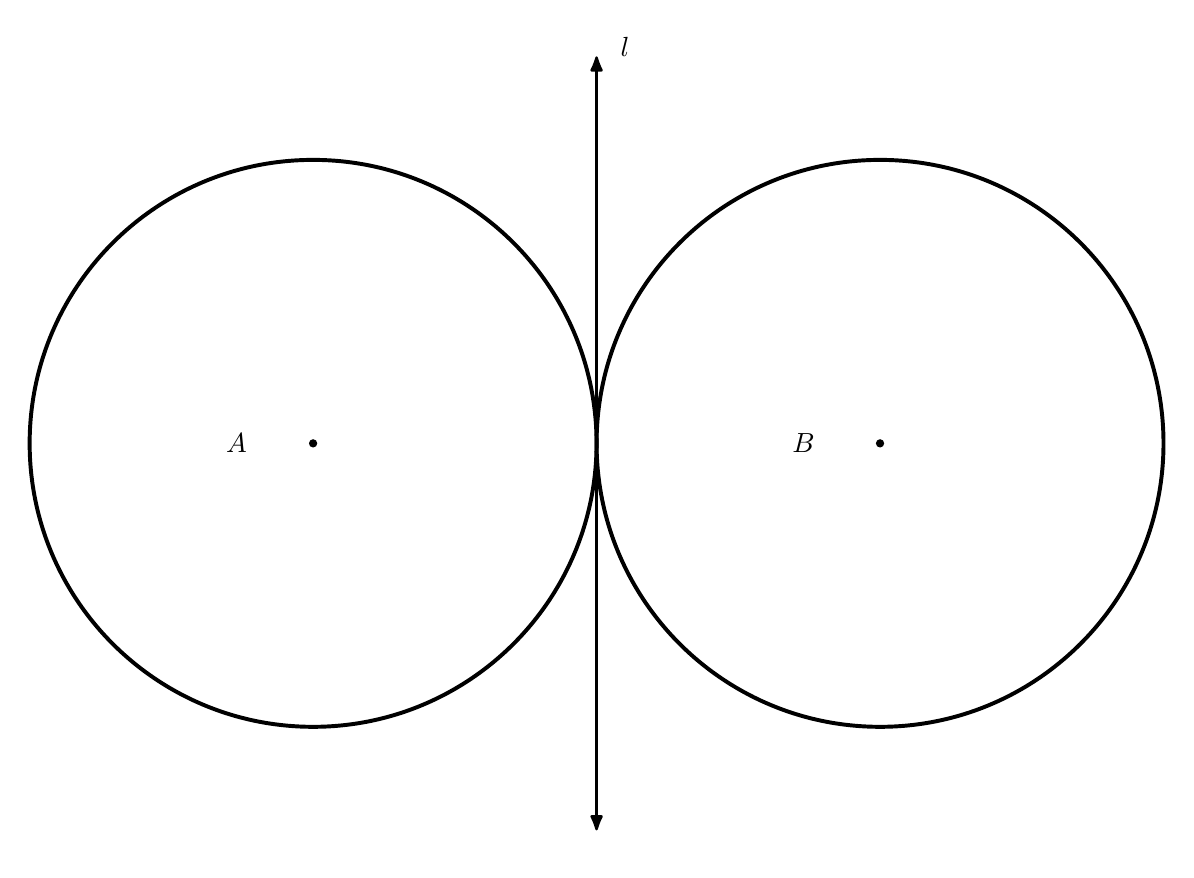
\begin{tikzpicture}[remember picture, %overlay,  
%baseline = (current bounding box.south)
]  

\coordinate (a) at (0,0); 

\draw[line width=0.5mm] (a) node[circle, fill=black, inner sep=0pt, outer sep=0pt, minimum size=3pt] {} circle [radius=\radA];

\node(a-label) at ($(a)+(180:0.27*\radA)$) {$  A$};

\node (b) at ($(a)+(0:\radA+\radB)$) {};

\draw[line width=0.5mm] (b) node[circle, fill=black, inner sep=0pt, outer sep=0pt, minimum size=3pt] {} circle [radius=\radB];

\node(b-label) at ($(b)+(180:0.27*\radA)$) {$  B$}; 

\node (int) at ($(a)+(0:\radA)$) {};

\node (c) at ($(int)+(90:0.7*\radA+0.7*\radB)$) {};

\node (d) at ($(int)+(-90:0.7*\radA+0.7*\radB)$) {};

\node (l) at ($(c)+(0:0.1*\radA)$) {$l$};

\draw[line width=0.3mm, <->, >={Latex[round]}] (c)--(d); 

\end{tikzpicture}

 
2. 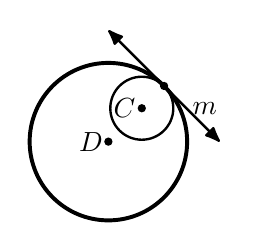
\begin{tikzpicture}[ 
remember picture, %overlay, 
baseline = (current bounding box.south)
] 

\def\radD{1cm}

\def\radC{0.4cm}

\coordinate (d) at (0,0); 

\draw[line width=0.5mm] (d) node[circle, fill=black, inner sep=0pt, outer sep=0pt, minimum size=3pt] {} circle [radius=\radD];

\node(d-label) at ($(d)+(180:0.22*\radD)$) {$  D$};

\draw ($(d)+(45:\radD)$) node[circle, fill=black, inner sep=0pt, outer sep=0pt, minimum size=3pt] (int) {} [];

\draw[line width=0.3mm, ->, >={Latex[round]}] (int) -- ($(int)!1!-90:(d)$);

\draw[line width=0.3mm, ->, >={Latex[round]}] (int) -- ($(int)!1!90:(d)$);

\node (c) at ($(int)!0.4!0:(d)$) {};

\draw[line width=0.3mm] (c) node[circle, fill=black, inner sep=0pt, outer sep=0pt, minimum size=3pt] {} circle [radius=\radC];

\node(c-label) at ($(c)+(180:0.22*\radD)$) {$  C$};

\node(m-label) at ($(c)+(0:0.8*\radD)$) {$  m$};

\end{tikzpicture}

\end{multicols}}
\end{minipage}}
\end{center}  


%}} 

%\newpage

%{\fontsize{38}{40}\fontfamily{pnc}\selectfont {

\def\currentdir{/storage/emulated/0/Documents/documents/latex/1920/Grade-10/2nd/tangent-lines-and-tangent-circles}

\vspace*{0.3cm}
\begin{center}
\scalebox{1}{
\noindent\begin{minipage}{\textwidth}

{\begin{multicols}{2}
3. \hspace*{1.5cm}
\begin{tikzpicture}[
remember picture, overlay, 
baseline = (current bounding box.west)
]  

\def\radE{0.5cm}

\def\radF{0.7cm}

\coordinate (intE) at (0,0); 

\coordinate (intF) at (1.5*\radF,0); 

\node(e) at ($(intE)+(90:\radE)$) {};

\draw[line width=0.5mm] (e) node[circle, fill=black, inner sep=0pt, outer sep=0pt, minimum size=3pt] {} circle [radius=\radE];

\node(e-label) at ($(e)+(50:0.3*\radF)$) {$  E$};

\draw[line width=0.3mm, <->, >={Latex[round]}] ($(intE) +(180:1.2*\radE)$) -- ($(intF) +(0:1.2*\radF)$);

\node(f) at ($(intF)+(-90:\radF)$) {};

\node(n) at ($(intF)+(15:1cm)$) {$  n$};

\draw[line width=0.5mm] (f) node[circle, fill=black, inner sep=0pt, outer sep=0pt, minimum size=3pt] {} circle [radius=\radF];

\node(f-label) at ($(f)+(-50:0.3*\radF)$) {$  F$};

\end{tikzpicture}

 %& 
4. \hspace*{1.5cm}\begin{tikzpicture}[remember picture, overlay, 
baseline = (current bounding box.north)
]  
 
\pgfmathsetmacro{\rone}{1} 

\pgfmathsetmacro{\rtwo}{0.6}
 
\pgfmathsetmacro{\mid}{\rone/(\rone + \rtwo)} 

\pgfmathsetmacro{\out}{\rone/(\rone - \rtwo)} 

\node[draw,circle,minimum size=2 * \rone cm,inner sep=0pt, line width=0.5mm] (c1) at (2*\rone,0) {}; 

\node[draw,circle,minimum size=2 * \rtwo cm,inner sep=0pt, line width=0.5mm] (c2) at (0,0) {}; 

\path (c1.center) -- node[coordinate,pos=\mid] (mid) {} (c2.center); 

\path (c1.center) -- node[coordinate,pos=\out] (out) {} (c2.center); 

\draw(c1.center) node  [circle, fill=black, inner sep=0pt, outer sep=0pt, minimum size=3pt] () {};

\draw(c2.center) node  [circle, fill=black, inner sep=0pt, outer sep=0pt, minimum size=3pt] () {};

\node(i-label) at ($(c1.center)+(180:0.22*\rone)$) {$  I$};

\node(h-label) at ($(c2.center)+(180:0.22*\rone)$) {$  H$};

\foreach \i in {1,2} 
\foreach \j in {1,2} 
\foreach \k in {mid,out} 
\coordinate (t\i\j\k) at (tangent cs:node=c\i,point={(\k)},solution=\j); 

\foreach \i in {1,2} 
\foreach \k in {mid,out} 
\draw[line width=0.3mm, <->, >={Latex[round]}] ($(t1\i\k)!-1cm!(t2\i\k)$) -- ($(t2\i\k)!-0.8cm!(t1\i\k)$); 

\node(p-label) at ($(t21mid)!-1cm!(t11mid)+(110:3pt) $) {$  p$};

\node(s-label) at ($(t22mid)!-1cm!(t12mid)+(-110:3pt) $) {$  s$};

\node(r-label) at ($(t21out)!-1cm!(t11out)+(-70:0.25*\rone) $) {$  r$};

\node(q-label) at ($(t22out)!-1cm!(t12out)+(70:0.25*\rone) $) {$  q$};

\end{tikzpicture}

 %\\
\end{multicols}}
\end{minipage}}
\end{center}   

\vspace*{1.3cm}
B. In $\odot{O}$, $\overline{CT}$, $\overline{ET}$ are tangent segments and $m$ is tangent to $\odot{O}$ at S. 
\begin{center}
\vspace*{-2ex}
\scalebox{1}{
\noindent\begin{minipage}{\textwidth}
{
\begin{enumerate}[label = \arabic*. ]
\item $m\angle{OCT}=$ \blank. 
\item $m\angle{OSI}=$ \blank. %\hspace*{8cm}\begin{tikzpicture}[remember picture, overlay
]

\def\rad{1.2cm}

\node[draw,circle,minimum size=2*\rad,inner sep=0pt, line width=0.5mm, outer sep=0] (c1) at (0,0) {}; 

\node(o-label) at ($(c1.center)+(150:0.22*\rad)$) {$  O$};

\coordinate (t) at (0,-3*\rad); 

\node(t-label) at ($(t)+(270:0.22*\rad)$) {$  T$};

\draw[line width=0.3mm] (c1.center) -- (tangent cs:node=c1, point={(t)}, solution=1) -- (t) -- (tangent cs:node=c1, point={(t)}, solution=2) -- cycle; 

\node(e-label) at ($(tangent cs:node=c1, point={(t)}, solution=1)+(-20:0.2*\rad)$) {$  E$};

\node(c-label) at ($(tangent cs:node=c1, point={(t)}, solution=2)+(200:0.2*\rad)$) {$  C$};

\coordinate (n) at (90:\rad); 

\node(n-label) at ($(n)+(90:0.2*\rad)$) {$  N$};

\coordinate (s) at (-90:\rad); 

\node(s-label) at ($(s)+(-90:0.2*\rad)$) {$  S$};

\node[circle, fill=black, inner sep=0pt, outer sep=0pt, minimum size=3pt] (i) at ($(s)+(180:\rad)$) {};

\coordinate (l) at ($(s)+(180:1.2*\rad)$); 

\node(i-label) at ($(i)+(90:0.2*\rad)$) {$  I$};

\coordinate (m) at ($(s)+(0:1.2*\rad)$); 

\node(l-label) at ($(m)+(90:0.2*\rad)$) {$m$};

\draw[line width=0.3mm] (n) -- (s); 

\draw[line width=0.3mm, <->, >={Latex[round]}] (l) -- (m); 

\end{tikzpicture}
 \vspace*{-2.5ex}
\item If $\overline{SN}=24$ units,  then $\overline{OE}=$ \blank. 
\item If $\overline{OS}=5$ units and $\overline{SI}=12$ units,\newline then $\overline{OI}=$ \blank. 
\item If $\overline{CT}=15$ units,  then $\overline{ET}=$ \blank. 
\item If $\overline{OC}=8$ units and\newline $\overline{ET}=15$ units,  then $\overline{OT}=$ \blank. 
\item If $\overline{OE}=11$ units, then $\overline{NS}=$ \blank. 
\item If $\overline{OS}=7$ units and  $\overline{OT}=25$ units,\newline then $\overline{CT}=$ \blank. 
\end{enumerate}  

\vspace*{-5cm}\hspace*{8.5cm}\begin{tikzpicture}[remember picture, overlay
]

\def\rad{1.2cm}

\node[draw,circle,minimum size=2*\rad,inner sep=0pt, line width=0.5mm, outer sep=0] (c1) at (0,0) {}; 

\node(o-label) at ($(c1.center)+(150:0.22*\rad)$) {$  O$};

\coordinate (t) at (0,-3*\rad); 

\node(t-label) at ($(t)+(270:0.22*\rad)$) {$  T$};

\draw[line width=0.3mm] (c1.center) -- (tangent cs:node=c1, point={(t)}, solution=1) -- (t) -- (tangent cs:node=c1, point={(t)}, solution=2) -- cycle; 

\node(e-label) at ($(tangent cs:node=c1, point={(t)}, solution=1)+(-20:0.2*\rad)$) {$  E$};

\node(c-label) at ($(tangent cs:node=c1, point={(t)}, solution=2)+(200:0.2*\rad)$) {$  C$};

\coordinate (n) at (90:\rad); 

\node(n-label) at ($(n)+(90:0.2*\rad)$) {$  N$};

\coordinate (s) at (-90:\rad); 

\node(s-label) at ($(s)+(-90:0.2*\rad)$) {$  S$};

\node[circle, fill=black, inner sep=0pt, outer sep=0pt, minimum size=3pt] (i) at ($(s)+(180:\rad)$) {};

\coordinate (l) at ($(s)+(180:1.2*\rad)$); 

\node(i-label) at ($(i)+(90:0.2*\rad)$) {$  I$};

\coordinate (m) at ($(s)+(0:1.2*\rad)$); 

\node(l-label) at ($(m)+(90:0.2*\rad)$) {$m$};

\draw[line width=0.3mm] (n) -- (s); 

\draw[line width=0.3mm, <->, >={Latex[round]}] (l) -- (m); 

\end{tikzpicture}
 \vspace*{5cm}
}
\end{minipage}}
\end{center}  
}}
\newpage

{\fontsize{36}{40}\fontfamily{pnc}\selectfont {
\def\currentdir{/storage/emulated/0/Documents/documents/latex/1920/Grade-10/2nd/tangent-lines-and-tangent-circles}

\def\myrad{1cm}

\textbf{Problem Set}

\vspce

Use the given figures to find the values of $x$ and $y$.

\begin{center}
\scalebox{1}{
\noindent\begin{minipage}{\textwidth}
{\begin{tabularx}{\textwidth}{XXX}
1. \begin{tikzpicture}[dot/.style={circle, fill=black, inner sep=0pt, outer sep=0pt, minimum size=3pt}]

\node[draw,circle,minimum size=2*\myrad,inner sep=0pt, line width=0.5mm, outer sep=0] (o) at (0,0) {}; 

\node(o-dot)[dot] at (o.center) {};

\node(o-label) at ($(o.center)+(180:0.27*\myrad)$) {$  O$};

\coordinate (t) at (2*\myrad,0); 

\node(58) at ($(t)+(190:0.5*\myrad)$) {$  58\degree$};

\draw[line width=0.3mm] (o.center) -- (tangent cs:node=o, point={(t)}, solution=1) -- (t) -- (tangent cs:node=o, point={(t)}, solution=2) -- cycle; 

\node(x-label) at ($(o)+(0:0.22*\myrad)$) {$  x$};

\end{tikzpicture}

 & 4. \begin{tikzpicture}[dot/.style={circle, fill=black, inner sep=0pt, outer sep=0pt, minimum size=3pt}]

\node[draw,circle,minimum size=2*\myrad,inner sep=0pt, line width=0.5mm, outer sep=0] (c1) at (0,0) {};

\node(o-dot)[dot] at (o.center) {};

\coordinate (a) at ($(o.center)+(90:\myrad) $); 

\coordinate (b) at ($(o.center)+(-90:\myrad) $); 

\coordinate (c) at ($(o.center)+(180:\myrad) $); 

\coordinate (ext) at ($(b)+(180:2*\myrad) $); 

\node(o-label) at ($(o.center)+(20:0.23*\myrad)$) {$  O$};

\node(x-label) at ($(a)+(-112:0.38*\myrad)$) {$  x$};

\node(y.label) at ($(b)+(150:0.48*\myrad)$) {\tiny $y$};

\node(45-label) at ($(ext)+(20:0.6*\myrad)$) {$  45\degree$};

\draw[line width=0.3mm] (b) -- (c) -- (ext) -- (b) -- (a) ; 

\draw[line width=0.3mm] (a) -- (c) ; 

\end{tikzpicture}

 & 7. \begin{tikzpicture}[dot/.style={circle, fill=black, inner sep=0pt, outer sep=0pt, minimum size=3pt}, dim-label/.style={fill=white, rectangle, inner sep=2pt, outer sep=0pt}]

\node[draw,circle,minimum size=2*\myrad,inner sep=0pt, line width=0.5mm, outer sep=0] (e) at (0,0) {};

\node(e-dot)[dot] at (e.center) {};

\coordinate (k) at ($(e.center) +(90:\myrad)$);

\node(k-label) at ($(k)+(90:0.18*\myrad)$) {$  K$};

\coordinate (a) at ($(e.center) + (180:\myrad)$);

\node(a-label) at ($(a)+(180:0.18*\myrad)$) {$  A$};

\coordinate (r) at ($(e.center) +(-90:\myrad)$);

\node(r-label) at ($(r)+(-90:0.18*\myrad)$) {$  R$};

\coordinate (g) at ($(a)+(90:\myrad) $);

\node(g-label) at ($(g)+(90:0.18*\myrad)$) {$  G$};

\coordinate (d) at ($(a)+(-90:\myrad) $);

\node(d-label) at ($(d)+(-90:0.18*\myrad)$) {$  D$};

\coordinate (o) at ($(k)+(0:1.3*\myrad) $);

\node(o-label) at ($(o)+(50:0.18*\myrad)$) {$  O$};

\coordinate (ext) at ($(a)+(180:0.4*\myrad) $);

\coordinate (u) at (tangent cs:node=e, point={(o)}, solution=2); 

\node(u-label) at ($(u)+(-40:0.22*\myrad)$) {$  U$};

\coordinate (guess1) at ($(o)!1.7!(u)$);

\coordinate (guess2) at ($(d)!1.88!(r)$);

\node(e-label) at ($(e.center)+(20:0.18*\myrad)$) {$  E$};

\draw[line width=0.3mm] (u) -- (o) -- (g) -- (d) -- (r);

\path[name path=line1.guess, line width=0.3mm] (u) -- (guess1); 

\path[name path=line2.guess, line width=0.3mm] (r) -- (guess2); 

\fill[red, name intersections={of=line1.guess and line2.guess, name=point}];

\draw[line width=0.3mm] (u) -- (point-1) -- (r) ; 

\node(l-label) at ($(point-1)+(-60:0.18*\myrad)$) {$  L$};

\draw[{Rays[n=2].Classical TikZ Rightarrow[]}-{Classical TikZ Rightarrow[].Rays[n=2]}, line width=0.3mm] ($(ext)+(90:\myrad+1pt)$) -- ($(ext)+(-90:\myrad+1pt)$);

\node[dim-label] (x-label) at ($(ext)+(90:0.3*\myrad)$) {\tiny $\text{x cm}$};

\node (8cm) at ($(g)+(20:0.5*\myrad)$) {\tiny 8 cm};

\node (16cm) at ($(o)+(-65:0.5*\myrad)$) {\tiny 16 cm};

\node (6cm) at ($(u)+(-70:0.5*\myrad)$) {\tiny 6 cm};

\node (12cm) at ($(r)+(200:0.5*\myrad)$) {\tiny 12 cm};
\end{tikzpicture}

 \\[-3ex]

2. \begin{tikzpicture}[dot/.style={circle, fill=black, inner sep=0pt, outer sep=0pt, minimum size=3pt}]

\node[draw,circle,minimum size=2*\myrad, inner sep=0pt, line width=0.5mm, outer sep=0] (o) at (0,0) [] {};

\node(o-dot)[dot] at (o.center) {};

\coordinate (ext) at ($(o.center)+(200:2*\myrad) $); 

\node(o-label) at ($(o.center)+(18:0.23*\myrad)$) {$  O$};

\node(42-label) at ($(ext)+(25:0.6*\myrad)$) {$  42\degree$};

\draw[line width=0.3mm] ($(tangent cs:node=o, point={(ext)}, solution=2)!2!0:(o.center)$) -- (ext) -- (tangent cs:node=o, point={(ext)}, solution=2) -- (o.center) ; 

\draw[line width=0.3mm] (o.center) -- ($(tangent cs:node=o, point={(ext)}, solution=2)!2!0:(o.center)$) ; 

\node(x-label) at ($(tangent cs:node=o, point={(ext)}, solution=2)!2!0:(o.center) + (163:0.5*\myrad) $) {$  x$};


\end{tikzpicture}

 & 5. \begin{tikzpicture}[dot/.style={circle, fill=black, inner sep=0pt, outer sep=0pt, minimum size=3pt}]

\node[draw,circle,minimum size=2*\myrad,inner sep=0pt, line width=0.5mm, outer sep=0] (c1) at (0,0) {};

\node(o-dot)[dot] at (o.center) {};

\coordinate (ext) at ($(o.center)+(0:2.4*\myrad) $); 

\node(o-label) at ($(o.center)+(180:0.22*\myrad)$) {$  O$};

\node(x-label) at ($(tangent cs:node=o, point={(ext)}, solution=1)+(-60:0.25*\myrad)$) {\tiny $x$};

\node(y-label) at ($(o.center)+(32:0.22*\myrad)$) {\tiny $y$};

\node(z-label) at ($(tangent cs:node=o, point={(ext)}, solution=2)+(60:0.25*\myrad)$) {\tiny $z$};

\node(35-label) at ($(ext)+(169:0.88*\myrad)$) {\tiny $35\degree$};

\draw[line width=0.3mm] (ext) -- (o.center) -- (tangent cs:node=o, point={(ext)}, solution=1) ; 

\draw[line width=0.3mm] (tangent cs:node=o, point={(ext)}, solution=1) -- (tangent cs:node=o, point={(ext)}, solution=2) ; 

\draw[line width=0.3mm] (tangent cs:node=o, point={(ext)}, solution=2) -- (o.center) ; 

\draw[line width=0.3mm] ($(ext)!1.5!(tangent cs:node=o, point={(ext)}, solution=1)$) -- (ext) -- ($(ext)!1.5!(tangent cs:node=o, point={(ext)}, solution=2)$); 

\end{tikzpicture}

 & 8. \begin{tikzpicture}[dot/.style={circle, fill=black, inner sep=0pt, outer sep=0pt, minimum size=3pt}]

\node[draw,circle,minimum size=2*\myrad,inner sep=0pt, line width=0.5mm, outer sep=0] (o) at (0,0) {};

\node(o-dot)[dot] at (o.center) {};

\coordinate (a) at ($(o.center)+(-90:\myrad) $); 

\coordinate (ext) at ($(a)+(180:2*\myrad) $); 

\node(o-label) at ($(o.center)+(20:0.22*\myrad)$) {$  O$};

\node(x1-label) at ($(o.center)+(190:0.5*\myrad)$) {$x$};

\node(x2-label) at ($(o.center)+(-70:0.5*\myrad)$) {$x$};

\node(4) at ($(o.center)+(200:1.6*\myrad)$) {$  4$};

\node(8) at ($(a)+(190:\myrad)$) {$8$};

\draw[line width=0.3mm] (ext) -- (tangent cs:node=o, point={(ext)}, solution=1) -- (o.center) -- cycle; 

\end{tikzpicture}
 \\[-6ex]

3. \begin{tikzpicture}[dot/.style={circle, fill=black, inner sep=0pt, outer sep=0pt, minimum size=3pt}]

\node[draw,circle,minimum size=2*\myrad,inner sep=0pt, line width=0.5mm, outer sep=0] (o) at (0,0) {};

\node(o-dot)[dot] at (o.center) {};

\coordinate (ext) at ($(o.center)+(270:2*\myrad) $); 

\node(o-label) at ($(o.center)+(20:0.23*\myrad)$) {$  O$};

\node(x-label) at ($(ext)+(75:0.5*\myrad)$) {$  x$};

\node[rotate=-30](60-label) at ($(o.center)+(-50:0.5*\myrad)$) {$ 60\degree$};


\draw[line width=0.3mm] (ext) -- (tangent cs:node=o, point={(ext)}, solution=1) -- (o.center) -- cycle; 

\end{tikzpicture}

 & 6. \begin{tikzpicture}[dot/.style={circle, fill=black, inner sep=0pt, outer sep=0pt, minimum size=3pt}, dim-label/.style={fill=white, rectangle, inner sep=2pt, outer sep=0pt}]

\node[draw,circle,minimum size=2*\myrad,inner sep=0pt, line width=0.5mm, outer sep=0] (o) at (0,0) {};

\node(o-dot)[dot] at (o.center) {};

\coordinate(a) at ($(o.center) +(-90:\myrad)$);

\coordinate(b) at ($(o.center) + (0:\myrad)$);

\coordinate (ext) at ($(a)+(180:\myrad)$); 

\coordinate (ext2) at ($(b)+(90:\myrad)$); 

\coordinate (ext3) at ($(ext)+(90:2*\myrad)$); 

\coordinate (ext4) at ($(ext)+(0:2*\myrad)$); 

\coordinate (ext5) at ($(b)+(0:0.3*\myrad)$); 

\draw[line width=0.3mm] (ext) rectangle (ext2);

\begin{scope} [rotate=0]
\draw[line width=0.3mm] (ext) rectangle ++(0.22*\myrad,0.22*\myrad) node[transform shape]{};
\end{scope}

\begin{scope} [rotate=180]
\draw[line width=0.3mm] (ext2) rectangle ++(0.22*\myrad,0.22*\myrad) node[transform shape]{};
\end{scope}

\begin{scope} [rotate=-90]
\draw[line width=0.3mm] (ext3) rectangle ++(0.22*\myrad,0.22*\myrad) node[transform shape]{};
\end{scope}

\begin{scope} [rotate=90]
\draw[line width=0.3mm] (ext4) rectangle ++(0.22*\myrad,0.22*\myrad) node[transform shape]{};
\end{scope}

\node(o-label) at ($(o.center)+(180:0.23*\myrad)$) {$  O$};

\draw[line width=0.3mm] (o.center) -- (b) ;

\node(14) at ($(o.center)+(15:0.5*\myrad)$) {\tiny $\text{14 ft.}$}; 

\draw[{Rays[n=2].Classical TikZ Rightarrow[]}-{Classical TikZ Rightarrow[].Rays[n=2]}, line width=0.3mm] ($(ext5)+(90:\myrad+1pt)$) -- ($(ext5)+(-90:\myrad+1pt)$);

\node[dim-label] (x-label) at (ext5) {\tiny $\text{x ft.}$};

\end{tikzpicture}

 & \vspace*{-2cm} 9.\hspace*{1.5cm}\begin{tikzpicture}[dot/.style={circle, fill=black, inner sep=0pt, outer sep=0pt, minimum size=3pt}, 
remember picture, overlay, 
baseline = (current bounding box.south)
]  

\node[draw,circle,minimum size=2*\myrad,inner sep=0pt, line width=0.5mm, outer sep=0] (o) at (0,0) {};

\node(o-dot)[dot] at (o.center) {};

\coordinate (a) at ($(o.center)+(-90:\myrad) $); 

\coordinate (ext) at ($(a)+(0:2*\myrad) $); 

\node(o-label) at ($(o.center)+(90:0.22*\myrad)$) {$  O$};

\node(5) at ($(o.center)+(250:0.45*\myrad)$) {$  5$};

\node(x) at ($(o.center)+(-20:1.5*\myrad)$) {$x$};

\node(12) at ($(a)+(-10:1.1*\myrad)$) {$  12$};

\draw[line width=0.3mm] (ext) -- (tangent cs:node=o, point={(ext)}, solution=2) -- (o.center) -- cycle; 

\end{tikzpicture}


%\end{minipage} 
\\%[-2ex]

\end{tabularx}} 
\end{minipage}}
\end{center}




}}
\newpage

{\fontsize{36}{40}\fontfamily{pnc}\selectfont {
\input{ps-tangent-lines-and-tangent-circles-sol}

}}

\end{document}